\documentclass[a4paper,french,12pt]{article}
\usepackage[utf8]{inputenc}
\usepackage[T1]{fontenc}
\usepackage[french]{babel}
\usepackage{color}
\usepackage{fancybox}
\usepackage{shadow}
\usepackage{graphicx}
\usepackage{amsmath}
\usepackage{amssymb}
\usepackage{array}
\usepackage{latexsym}
\usepackage{geometry}
\geometry{hmargin=1cm,vmargin=1cm}
\usepackage{dsfont}

\title{\textbf{Éléments de logique, ensembles, applications}}
\date{}
\begin{document}

\maketitle
\section{Écritures symboliques}
\subsection{Quantificateurs}
\vspace{0.1cm}
\noindent
$\forall$ , se lit "pour tout". Exemple, $\forall$ x $\in$ $\mathbb{R}$, x > x - 1.\\
$\exists$, se lit "il existe". Exemple, $\exists$ x $\in$ $\mathbb{R}$ / x > 0.\\
$\exists$!, se lit "il existe un unique". Exemple, $\exists$! x $\in$ $\mathbb{R}$ / x - 1 = 0.\\

\subsection{Appartenance, inclusion}
\vspace{0.1cm}
\noindent
Vocabulaire et notations:\\
\indent Ensemble vide: \O \: ou \{\}\\
\indent Singleton: \{a\}\\
\indent Paire: \{a; b\} avec a $\neq$ b\\
\indent Couple: (a;b)\\
\\
Soit E un ensemble.\\
L'ensemble des couples d'éléments de E est noté $E \times E$ = $E^2$.
\begin{displaymath}
E \times E = \{ (a;b),\, a \in E,\, b \in E \}
\end{displaymath}
Plus généralement, $E^n = \{(a_1;a_2;...;a_n), \forall i \in \{1;...;n\}, a_i \in E\}$\\
\\
L'ensemble des parties de E est $\mathcal{P}(E)$.\\
Soit $E = \{a;b\}$ avec a $\neq$ b alors $\mathcal{P}(E) = \{ \{a\}; \{b\}; \{a;b\};$\O$\}$\\
On dit que $\{a\} \subset E$ et que $\{a\} \in \mathcal{P}(E)$.

\subsection{Implication, équivalences}
\vspace{0.1cm}
\noindent
L'implication se note $\Rightarrow$ .\\
L'équivalence se note $\Leftrightarrow$ .\\
\\
Attention $\Rightarrow$ ne signifie pas la même chose que "donc".\\
Soit P et Q deux phrases.\\
P donc Q signifie: P est vraie donc Q est vraie.\\
P$\Rightarrow$Q signifie: si P est vraie alors Q est vraie.\\
\\
Exemples:\\
$\forall x \in \mathbb{R}$, $x\geq 2$ donc $x^2 \geq 4$.\\
$\forall x \in \mathbb{R}$, $x \geq 2$ $\Rightarrow$ $x^2 \geq 4$.\\
\\
Tables de vérité:\\
\\
\begin{tabular}{|c|c|c|c|}
\hline
P & Q & P$\Rightarrow$Q & P donc Q\\
\hline
V & V & V & V\\
\hline
V & F & F & F\\
\hline
F & V & V & F\\
\hline
F & F & V & F\\
\hline
\end{tabular}
\\
\\
Ne pas confondre: "P$\Leftrightarrow$Q" et "P et Q".\\
"P$\Leftrightarrow$Q" signifie que P et Q sont vraies ou fausses en même temps.\\
"P et Q" signifie que P est vraie et Q est vraie.

\section{Différents types de raisonnement}

\subsection{Raisonnement déductif}

Le schéma du raisonnement déductif est le suivant:\\
\\
\textcolor{red}{
\shabox{
Quand P est une proposition vraie, et P$\Rightarrow$Q est une proposition vraie, on peut affirmer que Q est une proposition vraie.
}}\\
\\
C'est un raisonnement de base qui sera souvent utilisé. Il faudra tout de même veiller à ne pas confondre "P$\Rightarrow$Q est vraie" et "P est vraie et P$\Rightarrow$Q est vraie", la seconde phrase permet d'affirmer que Q est vraie, pas l'autre.

\subsection{Raisonnement par l'absurde}

Lorsque l'on veut montrer qu'une proposition P est vraie, on suppose que sa négation $\bar{P}$ est vraie et on montre que cela entraine une proposition fausse.\\
Cela se résume de la manière suivante:\\
\\
\textcolor{red}{
\shabox{
Quand $\bar{P} \Rightarrow Q$ est une proposition vraie, et Q est une proposition fausse, on peut affirmer que P est une proposition vraie.
}}\\
\\
Exemple:\\
Montrons que $\sqrt{2}$ est irrationnel.\\
Supposons par l'absurde que $\sqrt{2} \in \mathbb{Q}$. Il existe alors deux entiers naturels non nuls a et b tels que $\sqrt{2} = \dfrac{a}{b}$ ou encore $a^2 = 2b^2$. (a est donc supérieur à 2)\\
En utilisant la décomposition en facteurs premiers, il vient que le nombre premier 2 apparaît avec un exposant pair ($2b^2$ étant pair).\\
Ainsi si $a = 2^{\alpha} \times \dots$ alors $a^2 = 2^{2\alpha} \times \dots$ mais l'exposant du nombre 2 est impair dans $2b^2$ ie si $b = 2^{\beta} \times \dots$ alors $b^2 = 2^{2\beta + 1} \times \dots$.\\
Or la décomposition en facteurs premiers est unique, donc l'égalité des nombres $a^2$ et $2b^2$ n'est pas possible, ainsi l'hypothèse de départ est fausse, donc $\sqrt{2} \notin \mathbb{Q}$.

\subsection{Raisonnement par contraposition}

Le principe de ce type de raisonnement est le suivant:\\
\\
\textcolor{red}{
\shabox{
Pour montrer que $P\Rightarrow Q$ est une proposition vraie, il faut et il suffit que de montrer que $\bar{Q} \Rightarrow \bar{P}$ est une proposition vraie.
}}\\
\\
Exemple:\\
Soient k et k' deux entiers naturels non nuls. Montrons que $\{ kk' = 1 \Rightarrow k = k' = 1 \}$.\\
Supposons que $k\neq 1$ ou $k' \neq 1$. On a donc $(k \geq 2 \: et\: k'\geq 1)$ ou bien $(k\geq 1 \: et \: k'\geq 2)$.\\
Dans les deux cas, $kk' \geq 2$ donc $kk' \neq 1$.\\
Ainsi, ($k\neq 1$ ou $k'\neq 1$) $\Rightarrow$ ($kk'\neq 1$).

\subsection{Raisonnement par récurrence}

\noindent Récurrence simple:\\
\textcolor{red}{
\shabox{
\noindent
Soit $P_n$ une assertion dépendant de l'entier naturel n et $n_0 \in \mathbb{N}$.\\
Si $\left\lbrace
\begin{array}{l}
(i) \: P_{n_0} \: est \: vraie \\
(ii) \: \forall n \geq n_0: \: P_n \Rightarrow P_{n+1} \: est \: vraie
\end{array}
\right.$
\\
alors $\forall n \geq n_0,\: P_n$ est vraie
}}\\
\\
\noindent Récurrence forte:\\
\textcolor{red}{
\shabox{
\noindent
Soit $P_n$ une assertion dépendant de l'entier naturel n et $n_0 \in \mathbb{N}$.\\
Si $\left\lbrace
\begin{array}{l}
(i) \: P_{n_0} \: est \: vraie \\
(ii) \: \forall n \geq n_0: \: P_{n_0},P_{n_0+1},\dots P_n \Rightarrow P_{n+1} \: est \: vraie
\end{array}
\right.$
\\
alors $\forall n \geq n_0,\: P_n$ est vraie
}}

\subsection{Raisonnement par analyse-synthèse}

\noindent
\textcolor{red}{
\shabox{
Le raisonnement par analyse-synthèse est un type de raisonnement mathématique permettant de démontrer l'existence et l'unicité d'un objet vérifiant des propriétés données. Il y a donc deux étapes:\\
\indent 1) Analyse:\\
on suppose que l'objet existe et on essaie de trouver des conditions nécessaires que doit vérifier cet objet. Ainsi, on prouve que si l'objet existe, il aura une certaine forme (cela nous assure l'unicité).
\indent 2) Synthèse:\\
on considère l'objet identifié dans la partie analyse, et on vérifie qu'il a bien les propriétés voulues (cela assure l'existence)
}}\\
\\
Exercice:\\
Résoudre sur $\mathbb{R}$ l'équation $x=\sqrt{2-x}$.\\
\\
Analyse:\\
Si x est solution de cette équation alors en élevant au carré on obtient $x^2=2-x$. Donc x est solution de $x^2+x-2=0$, donc $x=-2$ ou $x=1$. On a donc justifié que si x est solution alors x vaut -2 ou 1.\\
Synthèse:\\
On vérifie que les valeurs trouvées précédemment sont solutions et on constate que -2 n'est pas solution et que 1 est solution. Donc la seule solution est $x=1$.

\section{Ensembles}

\noindent
\textcolor{red}{
\shabox{
\noindent
\textbf{Définition:}\\
Soient E et F deux ensembles, on dit que F est inclus dans E (ou queF est une partie de E ou que F est un sous-ensemble de E) et on note $F \subset E$ lorsque tout élément de F est un élément de E.\\
En notation mathématique cela donne, $\forall x\in F, \: x\in E$.
}}\\
\\
\\
\textcolor{red}{
\shabox{
\noindent
\textbf{Définition:}\\
Soient E un ensemble, A et B deux parties de E. On définit les ensembles:\\
$A\cup B$ = $\{ x \in E \; / \; x \in A\; ou \; x\in B\}$ c'est la réunion des ensembles A et B.\\
$A\cap B$ = $\{ x\in E \; / \; x\in A \; et \; x \in B\}$ c'est l'intersection des ensembles A et B.
}}\\
\\
\begin{figure}[h]
    \begin{minipage}[c]{.5\linewidth}
        \centering
        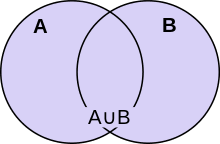
\includegraphics[scale=0.6]{chap1_image1}
        \caption{Réunion}
    \end{minipage}
    \hfill%
    \begin{minipage}[c]{.5\linewidth}
        \centering
        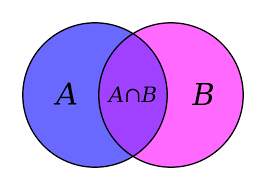
\includegraphics[scale=0.6]{chap1_image2}
        \caption{Intersection}
    \end{minipage}
\end{figure}


%\begin{tabular}{c|c}
%\begin{figure}[h]
%\begin{center}
%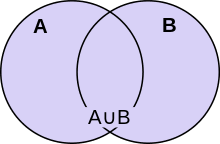
\includegraphics[scale=0.6]{chap1_image1}
%\end{center}
%\end{figure}

%\begin{figure}[h]
%\begin{center}
%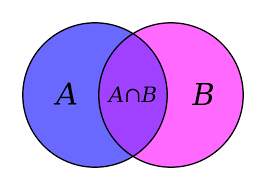
\includegraphics[scale=0.6]{chap1_image2}
%\end{center}
%\end{figure}
%\end{tabular}
\noindent
\textcolor{red}{
\shabox{
\noindent
\textbf{Propriétés:}\\
$\forall (A,B,C) \in \mathcal{P}(E)^3$, on a\\
Commutativité:\\
\indent (1a) $A\cup B$ = $B\cup A$ \\
\indent (1b) $A\cap B$ = $B\cap A$\\
Associativité:\\
\indent (2a) $(A\cup B)\cup C$ = $A\cup (B\cup C)$ \\
\indent (2b) $(A\cap B) \cap C$ = $A\cap (B\cap C)$.\\
Distributivité:\\
\indent (3a) $A\cap (B\cup C)$ = $(A\cap B) \cup (A\cap C)$\\
\indent (3b) $A \cup (B\cap C)$ = $(A\cup B) \cap (A\cup C)$
}}\\
\\
Démonstration du (3a) à faire.\\
\\
\textcolor{red}{
\shabox{
\noindent
\textbf{Définition:}\\
Soit E un ensemble, A une partie de E. \\
On définit l'ensemble: $C^E_A = \bar{A} = E\textbackslash A = \{ x \in E \; / \; x\notin A \}$.\\
On l'appelle complémentaire de A dans E.
}}\\
\\
\\
\textcolor{red}{
\shabox{
\noindent
\textbf{Propriétés:}\\
Soient E un ensemble, A et B deux parties de E, alors:\\
\indent (i) $\bar{\bar{A}} = A$\\
\indent (ii) $\bar{A\cup B} = \bar{A} \cap \bar{B}$\\
\indent (iii) $\bar{A\cap B} = \bar{A} \cup \bar{B}$
}}\\
\\
Démo à faire??

\section{Applications}

\subsection{Généralités}

\noindent
\textcolor{red}{
\shabox{
\noindent
\textbf{Définition:}\\
Soient E et F des ensembles et G une partie de E$\times $F.\\
On dit que E, F et G définissent une application ssi
$\forall x\in E, \: \exists ! \, y\in F \, / \, (x;y)\in G$.\\
G est appelé graphe de cette application.\\
L'ensemble des applications de E dans F est noté $\mathcal{F}(E,F)$ ou encore $F^E$.
}}\\
\\
Remarque:\\
Il y a une forte analogie entre "applications" et "fonctions", par conséquent le vocabulaire utilisé sera identique.\\
\\
Exemple:\\
E=\{a;b;c;d\} un ensemble ayant 4 éléments distincts, F=\{1;2;3;4;5;6\} et G=\{(a;3);(b;5);(c;3);(d;1)\}.\\
G est le graphe d'une application f:E$\rightarrow$F telle que 
a$\rightarrow$3; b$\rightarrow$5; c$\rightarrow$3 et d$\rightarrow$1
\\
\\
\textcolor{red}{
\shabox{
%\noindent
\textbf{Définition:}\\
On appelle identité de E et l'on note $Id_E$ l'application $Id_E$:
$\left\lbrace
\begin{array}{l}
E \rightarrow E\\
x \rightarrow x
\end{array}
\right.$
}}\\
\\
\\
\textcolor{red}{
\shabox{
\noindent
\textbf{Définition:}\\
Soient E un ensemble et A une partie de E. On appelle fonction indicatrice de A la fonction notée $\mathds{1}_A$ définie par:
$\left\lbrace
\begin{array}{l}
E \rightarrow E\\
x \rightarrow
   \left\lbrace
   \begin{array}{l}
   1 \; si \; x \in A \\
   0 \; sinon
   \end{array}
   \right.
\end{array}
\right.$
}}\\
\\
Exemples:\\
Représenter graphiquement les fonctions indicatrices suivantes: $\mathds{1}_{[0;1]}$ et $\mathds{1}_{\mathbb{Z}}$.\\
\\
\textcolor{red}{
\shabox{
\noindent
\textbf{Définition:}\\
Soient E et F deux ensembles non vides, f une application de E dans F et A une partie non vide de E, on appelle restriction de f à A et on note $f_{/A}$ l'application définie par
$\left\lbrace
\begin{array}{l}
A \rightarrow F\\
x \rightarrow f(x)
\end{array}
\right.$
}}\\
\\
\textcolor{red}{
\shabox{
\noindent
\textbf{Définition:}\\
Soient E et F deux ensembles non vides, f une application de E dans F et soit E' un ensemble tel que $E\subset E'$.\\
Un prolongement de f à E' est une application $f_1$ de E' vers F telle que $\forall x\in E,\; f_1(x)=f(x)$. $f_1(x)$ coïncide avec f sur E.
}}\\
\\
Exemple:\\
$f:x \rightarrow \dfrac{sin(x)}{x}$ est définie sur $\mathbb{R}^*$.\\
$f_1$:
$\left\lbrace
\begin{array}{l}
\mathbb{R} \rightarrow \mathbb{R}\\
x \rightarrow \frac{sin(x)}{x}\\
0 \rightarrow 1
\end{array}
\right.$
$f_1$ est un prolongement par continuité de f à $\mathbb{R}$.

\subsection{Injections, surjections, bijections}

\noindent
\textcolor{red}{
\shabox{
\noindent
\textbf{Définition:}\\
Soient E et F deux ensembles non vides et $f\in F^E$.\\
On dit que f est une injection (ou application injective) de E dans F lorsque tout élément de F possède au plus un antécédent.\\
De manière mathématique, on dit que f est une injection de E dans F ssi\\
\begin{minipage}{\linewidth}
\centering $\forall (x_1;x_2)\in E\times E, \; f(x_1)=f(x_2) \Rightarrow x_1 = x_2$
\end{minipage}\\
ou encore par contraposée,\\
\begin{minipage}{\linewidth}
\centering $\forall (x_1;x_2)\in E\times E, \; x_1\neq x_2 \Rightarrow f(x_1) \neq f(x_2)$
\end{minipage}
}}\\
\begin{figure}[h]
	\begin{center}
		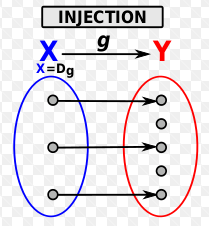
\includegraphics[scale=0.6]{chap1_image3}
	\end{center}
\end{figure}
\\
Exemples:\\
Les applications suivantes définies de $\mathbb{R}$ dans $\mathbb{R}$ sont-elles injectives? $f_1(x)=2x+1$ et $f_2(x)=x^2$.\\
\\
\textcolor{red}{
\shabox{
\noindent
\textbf{Définition:}\\
Soient E et F deux ensembles non vides et $f\in F^E$.\\
On dit que f est une surjection (ou application surjective) de E dans F lorsque tout élément de F possède au moins un antécédent.\\
De manière mathématique, on dit que f est une surjection de E dans F ssi\\
\begin{minipage}{\linewidth}
\centering $\forall y\in F, \; \exists \; x\in E \; / \; y=f(x)$
\end{minipage}
}}\\
\begin{figure}[h]
	\begin{center}
		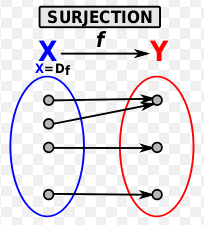
\includegraphics[scale=0.6]{chap1_image4}
	\end{center}
\end{figure}
\\
Exemple:\\
La fonction $f:x \rightarrow x^2$ est-elle surjective sur $\mathbb{R}$? sur $\mathbb{R}_+$?\\
\\
\textcolor{red}{
\shabox{
\noindent
\textbf{Définition:}\\
Soient E et F deux ensembles non vides et $f\in F^E$.\\
On dit que f est une bijection (ou application bijective) de E dans F lorsque tout élément de F possède un unique antécédent.\\
De manière mathématique, on dit que f est une bijection de E dans F ssi\\
\begin{minipage}{\linewidth}
\centering $\forall y\in F, \; \exists ! \; x\in E \; / \; y=f(x)$
\end{minipage}
}}\\
\\
Remarque:\\
Une application qui est à la fois injective et surjective est aussi bijective.\\
\begin{figure}[h]
	\begin{center}
		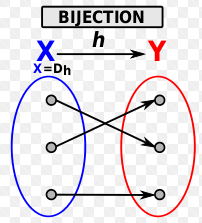
\includegraphics[scale=0.6]{chap1_image5}
	\end{center}
\end{figure}

\noindent
\textcolor{red}{
\shabox{
\noindent
\textbf{Définition:}\\
Soit f une bijection de E dans F, alors par définition tout élément de F possède un unique antécédent de E par f.\\
On appelle bijection réciproque de f et on note $f^{-1}$, l'application de F dans E qui à tout élément y de F fait correspondre son antécédent dans E par f, ainsi: $f^{-1}$:
$\left\lbrace
\begin{array}{l}
F \rightarrow E\\
y \rightarrow x \; tel \; que \; f(x)=y
\end{array}
\right. $\\
En résumé, $\forall (x;y)\in E\times F,\; y=f(x) \Leftrightarrow x=f^{-1}(y)$.
}}

\subsection{Composée d'applications}

\noindent
\textcolor{red}{
\shabox{
\noindent
\textbf{Définition:}\\
Soient E, F et G trois ensembles non vides, f une application de E dans F, g une application de F dans G.\\
On appelle composée des applications f et g et on note $g\circ f$ l'application définie par\\
$\left\lbrace
\begin{array}{l}
E \rightarrow G\\
x \rightarrow g(f(x))
\end{array}
\right. $
}}\\
\\
\textcolor{red}{
\shabox{
\noindent
\textbf{Propriété:}\\
Soient E, F, G et H des ensembles non vides, $f\in F^E$, $g\in G^F$ et $h\in H^G$, alors: $h\circ (g\circ f)=(h\circ g)\circ f$.
}}\\
\\
Démonstration:\\
$(h\circ (g\circ f))(x)=h((g\circ f)(x))=h(g(f(x)))=(h\circ g)(f(x))=((h\circ g)\circ f)(x)$\\
\\
\textcolor{red}{
\shabox{
\noindent
\textbf{Propriété:}\\
Soit f une bijection de E dans F et $f^{-1}$ sa bijection réciproque, alors: $f^{-1}\circ f = Id_E$ et $f\circ f^{-1} = Id_F$.
}}\\
\\
Démonstration à faire?\\
\\
\textcolor{red}{
\shabox{
\noindent
\textbf{Propriétés:}\\
1) La composée de deux injections est une injection.\\
2) La composée de deux surjections est une surjection.\\
3) La composée de deux bijections est une bijection.
}}\\
\\
Soient E, F et G des ensembles, $f\in F^E$ et $g\in G^F$.\\
\\
Démonstration du 1):\\
On suppose que f et g sont injectives et on montre que $g\circ f$ est injective.\\
Soit $(x_1;x_2)\in E^2$, on veut montrer que $(g\circ f)(x_1)=(g\circ f)(x_2) \Rightarrow x_1=x_2$.\\
On suppose que $(g\circ f)(x_1)=(g\circ f)(x_2)$ ainsi $g(f(x_1))=g(f(x_2))$.\\
On a alors $f(x_1)=f(x_2)$ puisque g est injective, ensuite il vient que $x_1=x_2$ puisque f est injective. Conclusion, $g\circ f$ est injective.\\
\\
Démonstration du 2):\\
On suppose que f et g sont surjectives et on montre que $g\circ f$ est surjective.\\
Il faut donc prouver que $\forall z\in G, \; \exists \; x\in E \; / \; z=(g\circ f)(x)$.\\
Soit $z\in G$ quelconque, $\exists y\in F \; / \; g(y)=z$ car g est surjective.\\
Soit y ainsi choisi, $\exists \; x\in E \; / \; f(x)=y$ car f est surjective.\\
Soit x ainsi choisi, on a $(g\circ f)(x)=g(f(x))=g(y)=z$. Ainsi z a bien un antécédent par $g\circ f$.\\
Conclusion, $g\circ f$ est surjective.\\
\\
Démonstration du 3):\\
C'est une conséquence des points 1) et 2).

\subsection{Image, image réciproque d'une partie}

\noindent
\textcolor{red}{
\shabox{
\noindent
\textbf{Définitions:}\\
Soient E et F deux ensembles non vides et $f\in F^E$.\\
Soit A une partie de E, on appelle image directe de A par f et on note f(A) l'ensemble:\\
\begin{minipage}{\linewidth}
\centering $\{ f(x)/x\in A\} = \{ y\in F \; tel\; que \; \exists \, x\in A, \; y=f(x)\}$.
\end{minipage}
\\
Soit B une partie de F, on appelle image réciproque de B par f et on note $f^{-1}(B)$ l'ensemble:\\
\begin{minipage}{\linewidth}
\centering $\{x\in E \, / \, f(x)\in B\}$.
\end{minipage}
}}

\subsection{Relations}

\noindent
\textcolor{red}{
\shabox{
\noindent
\textbf{Définition:}\\
Soit E un ensemble non vide.\\
Une relation $\mathcal{R}$ sur l'ensemble E est un couple (E,G) où G est une partie du produit cartésien $E\times E$.\\
On notera $x\mathcal{R} y$ au lieu de noter $(x,y)\in G$.
}}\\
\\
\textcolor{red}{
\shabox{
\noindent
\textbf{Définitions:}\\
Soit E un ensemble non vide, $\mathcal{R}$ une relation sur E.\\
On dit que $\mathcal{R}$ est une relation d'équivalence lorsqu'elle vérifie les trois conditions suivantes:\\
(i) $\forall x\in E,\; x\mathcal{R}x$. On dit que $\mathcal{R}$ est réflexive.\\
(ii) $\forall (x,y)\in E\times E$, si $x\mathcal{R}y$ alors $y\mathcal{R}x$. Dans ce cas, $\mathcal{R}$ est dite symétrique.\\
(iii) $\forall (x,y,z)\in E^3$, si $x\mathcal{R}y$ et $y\mathcal{R}z$ alors $x\mathcal{R}z$. On dit que $\mathcal{R}$ est transitive.
}}\\
\\
Exemples:\\
1) La relation "$\leq$" est réflexive alors que "<" ne l'est pas.\\
2) Les relations "=" et "$\Leftrightarrow$" sont symétriques.\\
3) Les relations "$\leq$" et "$\Rightarrow$" sont transitives.\\
\\
\textcolor{red}{
\shabox{
\noindent
\textbf{Définition:}\\
Soit E un ensemble non vide, $\mathcal{R}$ une relation sur E et $x\in E$.\\
On appelle classe d'équivalence de x et on note $C_x=\{y\in E\; / \; y\mathcal{R}x\}$.\\
Un élément quelconque de $C_x$ est appelé représentant de cette classe.
}}\\
\\
\textcolor{red}{
\shabox{
\noindent
\textbf{Définition:}\\
Soit E un ensemble non vide, $\mathcal{R}$ une relation sur E.\\
$\mathcal{R}$ est antisymétrique ssi $\forall (x,y)\in E^2,\; (x\mathcal{R}y\; et\; y\mathcal{R}x) \Rightarrow x=y$.
}}\\
\\
Exemple:\\
Les relations "$\leq$" et "=" sont antisymétriques.\\
\\
\textcolor{red}{
\shabox{
\noindent
\textbf{Définitions:}\\
Soit E un ensemble non vide, $\mathcal{R}$ une relation sur E.\\
Si $\mathcal{R}$ est réflexive, antisymétrique et transitive alors on dit que $\mathcal{R}$ est une relation d'ordre.\\
$\mathcal{R}$ est une relation d'ordre total ssi $\forall (x,y)\in E^2,\; x\mathcal{R}y \; ou \; y\mathcal{R}x$.\\
$\mathcal{R}$ est une relation d'ordre partiel ssi $\exists (x,y)\in E^2,\; / \; non(x\mathcal{R}y) \; et \; non(y\mathcal{R}x)$.
}}\\
\\
Exemples:\\
1) "$\leq$" est une relation d'ordre total dans $\mathbb{R}$.\\
2) "divise" est une relation d'ordre partiel dans $\mathbb{N}$.\\
\\
\textcolor{red}{
\shabox{
\noindent
\textbf{Définition:}\\
Soit $\alpha \in \mathbb{R}$, on dit que deux réels x et y sont congrus modulo $\alpha$ et on note $x \equiv y(\alpha)$ lorsqu'il existe un entier relatif k tel que : $x-y=k\alpha$.\\
Ainsi, $x \equiv y(\alpha) \; \Rightarrow \; \exists k\in \mathbb{Z} \; / \; x-y = k\alpha$.
}}\\
\\
\textcolor{red}{
\shabox{
\noindent
\textbf{Propriété:}\\
Soit $\alpha \in \mathbb{R}$, la relation $\mathcal{R}$ définie par $x\mathcal{R}y \; \Leftrightarrow \; x\equiv y(\alpha)$ est une relation d'équivalence sur $\mathbb{R}$.
}}\\
\\
Démonstration à faire?







\end{document}